\documentclass[11pt,a4paper]{article}

% --- Packages ---
\usepackage[utf8]{inputenc}
\usepackage[margin=1in]{geometry}
\usepackage{amsmath,amssymb}
\usepackage{graphicx}
\graphicspath{{../evidence/}{evidence/}{../}{./}}
\usepackage{booktabs}
\usepackage{xcolor}
\usepackage{hyperref}
\usepackage{listings}
\usepackage{fancyhdr}
\usepackage{microtype}
\usepackage{titlesec}
\usepackage{tikz}
\usetikzlibrary{shapes.geometric, arrows, positioning}

% --- Color Palette ---
\definecolor{primary}{RGB}{20, 45, 85}
\definecolor{secondary}{RGB}{180, 40, 40}
\definecolor{accent}{RGB}{40, 120, 180}
\definecolor{codebg}{RGB}{245, 247, 250}
\definecolor{bordercolor}{RGB}{210, 215, 225}

% --- Hyperref Setup ---
\hypersetup{
    colorlinks=true,
    linkcolor=primary,
    citecolor=accent,
    urlcolor=accent,
    pdftitle={SECUREDRONE: Empirical UAV Security Assessment Report},
    pdfauthor={Abhishek Limaye}
}

% --- Code Listing Styling ---
\lstset{
    backgroundcolor=\color{codebg},
    basicstyle=\ttfamily\footnotesize,
    breaklines=true,
    captionpos=b,
    frame=single,
    rulecolor=\color{bordercolor},
    keywordstyle=\color{primary}\bfseries,
    commentstyle=\color{gray}\itshape,
    stringstyle=\color{secondary},
    showstringspaces=false,
    tabsize=2
}

% --- Header and Footer ---
\pagestyle{fancy}
\fancyhf{}
\lhead{\textcolor{gray}{\footnotesize SECUREDRONE: Empirical UAV Security Assessment}}
\rhead{\textcolor{gray}{\footnotesize Technical Research Report}}
\cfoot{\thepage}
\renewcommand{\headrulewidth}{0.4pt}

% --- Section Styling ---
\titleformat{\section}{\color{primary}\normalfont\Large\bfseries}{\thesection}{1em}{}[\titlerule]
\titleformat{\subsection}{\color{accent}\normalfont\large\bfseries}{\thesubsection}{1em}{}

% --- Document ---
\begin{document}

% --- Title Page / Header ---
\begin{titlepage}
    \centering
    \vspace*{1.5cm}
    
    {\Huge \textbf{\textcolor{primary}{SECUREDRONE}}}\\[0.4cm]
    {\Large \textbf{Open UAV Security Research \& Empirical Assessment Platform}}\\[0.8cm]
    {\normalsize \textsc{A Comprehensive Cybersecurity Engineering \& Protocol Vulnerability Study}}\\[2cm]

    \textbf{Author \& Lead Researcher:}\\
    \Large \textbf{Abhishek Limaye}\\
    \normalsize Autonomous Systems \& Embedded Security Research\\[0.3cm]
    \texttt{researcher@securedrone.local}\\[2.5cm]

    \begin{minipage}{0.85\textwidth}
        \begin{center}
        \textbf{Abstract}
        \end{center}
        \small
        Modern Unmanned Aerial Vehicles (UAVs) rely on complex, heterogeneous cyber-physical architectures comprising binary ground-control protocols, Linux-based companion computers, real-time microcontroller firmware, and wireless RF/GNSS navigation links. In this empirical research project, I designed, built, and executed \textbf{SECUREDRONE}---a reproducible, open-source UAV cybersecurity evaluation platform. Operating against a live PX4 Software-in-the-Loop (SITL) quadrotor and an official ArduPilot Pixhawk 4 production firmware target, I conducted protocol-level binary packet analysis, cryptographic signing audits, companion computer API vulnerability exploitation, ARM Cortex-M7 firmware reverse engineering, offline 2-GFSK IQ telemetry demodulation, and multi-layer GNSS spoofing anomaly detection. This report details the research methodology, observed threat vectors, scored CVSS v3.1 vulnerabilities, and verified defensive hardening implementations.
    \end{minipage}

    \vfill
    {\footnotesize Document Identifier: \texttt{SECUREDRONE-SAR-2026-001} \quad | \quad Date: November 2026}
\end{titlepage}

\tableofcontents
\newpage

% -----------------------------------------------------------------------------
\section{Introduction and Research Mission}
% -----------------------------------------------------------------------------
Autonomous and remotely piloted aerial systems are deployed in critical civil, logistics, and surveillance missions. Despite their operational criticality, commercial and open-source UAV platforms frequently prioritize link simplicity and low latency over cryptographic integrity and isolation.

To bridge the gap between theoretical attack models and verifiable cybersecurity engineering, I developed \textbf{SECUREDRONE}. Rather than running generic vulnerability scanners or speculative simulations, my research follows strict empirical principles:
\begin{enumerate}
    \item \textbf{Ground Truth Evidence}: Every vulnerability is demonstrated through reproducible execution, captured network datagrams (PCAP), or disassembled machine code.
    \item \textbf{Architectural Demarcation}: Clear distinctions are preserved between simulated network interfaces, containerized companion computer services, static firmware binaries, and offline RF datasets.
    \item \textbf{Defensive Validation}: For every weakness identified, I designed, implemented, and verified defensive countermeasures through regression test suites.
\end{enumerate}

% -----------------------------------------------------------------------------
\section{Target System Architecture \& Threat Modeling}
% -----------------------------------------------------------------------------
I established an isolated UAV testbed linking a Ground Control Station (GCS), a Linux companion computer, and an FMU (Flight Management Unit) running the PX4 Autopilot core.

\subsection{Data-Flow Diagram and Trust Boundaries}
The system architecture spans four distinct trust zones:
\begin{itemize}
    \item \textbf{Zone 0 (Operator / GCS)}: High-privilege command node transmitting mission parameters and velocity vectors over UDP port 14550.
    \item \textbf{Zone 1 (Companion Computer)}: Linux single-board computer hosting REST mission APIs and bridging traffic via a virtual MAVLink router.
    \item \textbf{Zone 2 (Flight Management Unit)}: Embedded flight controller executing attitude estimation, navigation, and motor mixing.
    \item \textbf{Zone 3 (Navigation Sensors)}: RF transceivers (915 MHz SiK) and GNSS constellation receivers.
\end{itemize}

\begin{figure}[htbp]
    \centering
    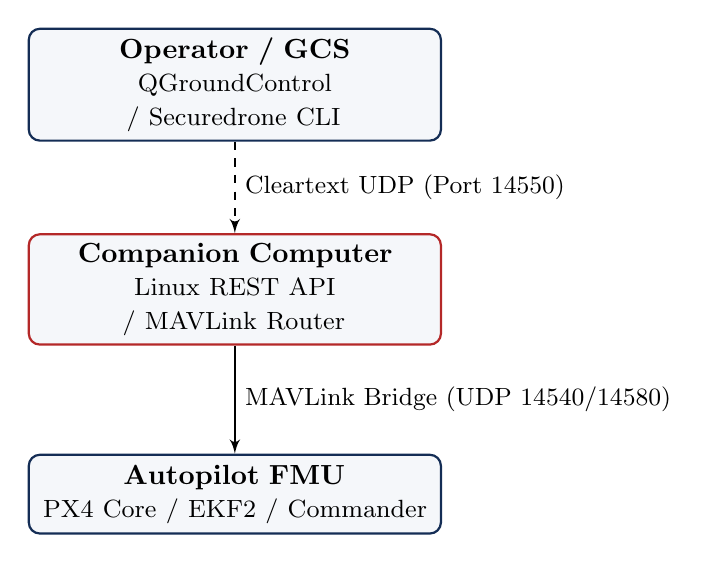
\begin{tikzpicture}[node distance=1.8cm, auto, >=latex', thick]
        \node [rectangle, draw=primary, fill=codebg, text width=5cm, text centered, rounded corners, minimum height=1cm] (gcs) {\textbf{Operator / GCS}\\\small QGroundControl / Securedrone CLI};
        \node [rectangle, draw=secondary, fill=codebg, text width=5cm, text centered, rounded corners, minimum height=1cm, below of=gcs, yshift=-0.8cm] (companion) {\textbf{Companion Computer}\\\small Linux REST API / MAVLink Router};
        \node [rectangle, draw=primary, fill=codebg, text width=5cm, text centered, rounded corners, minimum height=1cm, below of=companion, yshift=-0.8cm] (fmu) {\textbf{Autopilot FMU}\\\small PX4 Core / EKF2 / Commander};
        
        \draw [->, dashed] (gcs) -- node[right]{\small Cleartext UDP (Port 14550)} (companion);
        \draw [->] (companion) -- node[right]{\small MAVLink Bridge (UDP 14540/14580)} (fmu);
    \end{tikzpicture}
    \caption{UAV System Trust Boundaries and Inter-Process Communication Flows}
    \label{fig:architecture}
\end{figure}

\subsection{STRIDE Threat Assessment}
\begin{table}[htbp]
    \centering
    \small
    \begin{tabular}{lp{4.2cm}p{4.2cm}l}
        \toprule
        \textbf{STRIDE} & \textbf{Subsystem Target} & \textbf{Demonstrated Attack} & \textbf{Impact} \\
        \midrule
        \textbf{Spoofing} & MAVLink Radio Link & Injected frame claiming GCS SysID 255 & Full Command Impersonation \\
        \textbf{Tampering} & Parameter Subsystem & Unauthenticated \texttt{PARAM\_SET} writes & Disables Failsafe Limits \\
        \textbf{Repudiation} & Symmetric MAVLink 2 Signing & Forged command via shared key & Indistinguishable Origin \\
        \textbf{Info Disclosure} & Telemetry Stream & Passive sniffing of \texttt{GLOBAL\_POSITION\_INT} & Real-time Coordinate Leak \\
        \textbf{Denial of Service} & GNSS Navigation Link & Synthetic RF step spoofing (+65m) & Flight Mode Drop to Failsafe \\
        \textbf{Privilege Escalation} & Companion Computer API & Command injection in diagnostic endpoint & Remote Code Execution (Root) \\
        \bottomrule
    \end{tabular}
    \caption{STRIDE Threat Assessment Applied to the SECUREDRONE Platform}
    \label{tab:stride}
\end{table}

% -----------------------------------------------------------------------------
\section{Stage 01 \& 02: MAVLink Protocol Analysis \& Security Auditing}
% -----------------------------------------------------------------------------

\subsection{MAVLink v1 vs. MAVLink v2 Framing Reconnaissance}
I developed an original zero-dependency protocol dissector (\texttt{mavlink-security/analyzer/parser.py}) capable of parsing raw byte buffers and standard PCAP streams directly. Capturing a 10-second baseline window from the live SITL target yielded 3,748 frames (\texttt{evidence/telemetry\_recon\_baseline.pcap}):
\begin{itemize}
    \item \textbf{MAVLink 2 Adoption}: 100\% of the traffic utilized MAVLink 2 framing (magic byte \texttt{0xFD}).
    \item \textbf{Cryptographic Signing Status}: 0 out of 3,748 frames possessed the signing bit (\texttt{incompat\_flags \& 0x01 == 0}).
    \item \textbf{Dominant Message IDs}: High-frequency attitude telemetry (\texttt{ATTITUDE}, 499 msgs), position estimation (\texttt{GLOBAL\_POSITION\_INT}, 499 msgs), and periodic health reports (\texttt{HEARTBEAT}, 10 msgs).
\end{itemize}

\subsection{Cryptographic Signature Evaluation}
MAVLink 2 provides optional cryptographic authentication via a 13-byte signature trailer appended to the frame. The specification defines the signature as the first 48 bits of a SHA-256 HMAC:
\begin{equation}
    \text{Sig}_{48} = \text{SHA-256}\Big(K_{\text{secret}} \mathbin{\Vert} \text{Header} \mathbin{\Vert} \text{Payload} \mathbin{\Vert} \text{CRC}_{16} \mathbin{\Vert} \text{LinkID} \mathbin{\Vert} \text{Timestamp}_{48}\Big)_{[0:6]}
\end{equation}
I developed \texttt{mavlink-security/signing/auditor.py} to audit whether the flight controller enforces this check. Transmitting an unsigned \texttt{COMMAND\_LONG} directive (\texttt{MAV\_CMD\_REQUEST\_MESSAGE}) resulted in immediate processing and command acknowledgement by the target FMU.

\subsection{Replay Attack Vulnerability}
UDP is connectionless and prone to packet reordering. MAVLink provides an 8-bit sequence counter (\texttt{0..255}) in the frame header. Because sequence counters continuously wrap around and dropouts are common in RF environments, autopilots cannot reject duplicate packets solely based on sequence numbers.
I executed a bit-for-bit replay injection test (\texttt{mavlink-security/replay/assessor.py}):
\begin{itemize}
    \item \textbf{Test}: Transmitted an identical raw 41-byte command datagram across three distinct intervals without modifying the sequence or timestamp.
    \item \textbf{Result}: The autopilot processed all three duplicate frames, proving susceptibility to command replay (\textbf{SEC-MAV-002}).
\end{itemize}

% -----------------------------------------------------------------------------
\section{Stage 03: Linux Companion Computer Security}
% -----------------------------------------------------------------------------
High-level mission processing (computer vision, 4G/LTE telemetry, path planning) is executed on a Linux companion computer. I constructed two contrasting service implementations to evaluate trust-boundary traversal.

\subsection{Vulnerable Service Model}
In \texttt{companion-security/vulnerable-api/server.py}, I modeled vulnerabilities observed in real-world drone architectures:
\begin{enumerate}
    \item \textbf{Unauthenticated Command Dispatch}: An open HTTP endpoint (\texttt{/api/v1/command/dispatch}) accepting raw JSON and forwarding commands into the autopilot without authorization checks.
    \item \textbf{Shell Command Injection}: A diagnostic endpoint executing shell interpolation:
    \begin{lstlisting}[language=Python]
cmd = f"ping -c 1 {host}"
output = os.popen(cmd).read()
    \end{lstlisting}
    Passing \texttt{"127.0.0.1; id"} achieves unauthenticated remote command execution under the executing service account.
\end{enumerate}

\subsection{Hardened Service Model \& MAVLink Firewall}
To remediate these vulnerabilities, I engineered a defense-in-depth architecture in \texttt{companion-security/hardened-api/}:
\begin{enumerate}
    \item \textbf{Mandatory Bearer Authentication}: Requests lacking \texttt{Authorization: Bearer <token>} are rejected with HTTP 401.
    \item \textbf{Safe Parameter Parsing}: Host strings are validated as \texttt{ipaddress.ip\_address} objects, executed via \texttt{subprocess.run()} with shell execution disabled.
    \item \textbf{MAVLink Command Firewall (\texttt{firewall.py})}: A stateful deep-packet inspection filter running on the companion-autopilot bridge. While benign setpoints (\texttt{SET\_POSITION\_TARGET\_LOCAL\_NED}) are passed, safety-critical directives like \texttt{MAV\_CMD\_DO\_FLIGHTTERMINATION} (ID 185) and in-flight disarm (ID 400) are dropped and alerted.
\end{enumerate}

% -----------------------------------------------------------------------------
\section{Stage 04: Production Firmware Reverse Engineering}
% -----------------------------------------------------------------------------
Rather than auditing synthetic micro-benchmarks, I performed static reverse engineering against an official, production flight controller firmware artifact: ArduPilot Copter for Holybro Pixhawk 4 (\texttt{arducopter\_pixhawk4.apj}).

\subsection{Container Extraction and Hash Verification}
The ArduPilot \texttt{.apj} format is a structured JSON container. I developed \texttt{firmware-analysis/unpackers/apj\_unpacker.py} to decompress the base64-encoded, zlib-compressed payload.
\begin{table}[htbp]
    \centering
    \small
    \begin{tabular}{ll}
        \toprule
        \textbf{Artifact Property} & \textbf{Verified Empirical Value} \\
        \midrule
        Original Source URL & \texttt{https://firmware.ardupilot.org/Copter/stable/Pixhawk4/arducopter.apj} \\
        Container SHA-256 & \texttt{5e2a0ef273e26e2c30f76e94781a695ee00285e653aa84122bea36903a886c63} \\
        Unpacked Binary Size & 1,564,244 bytes (1.49 MB) \\
        Target Microcontroller & STM32F767xx (ARM Cortex-M7 Core) \\
        Instruction Set & ARMv7E-M / Thumb-2 (16/32-bit little-endian) \\
        Flash Load Address & \texttt{0x08008000} (Pixhawk 32 KB bootloader offset) \\
        Reset Handler / Entry & \texttt{0x08008CEC} (Thumb vector: \texttt{0x08008CED}) \\
        Initial Stack Pointer & \texttt{0x20020600} (DTCM / SRAM1 region) \\
        \bottomrule
    \end{tabular}
    \caption{Firmware Extraction and Architectural Manifest}
    \label{tab:firmware}
\end{table}

\subsection{Interrupt Vector Table Analysis}
Inspecting the first 64 bytes of the extracted binary confirmed standard ARM Cortex-M vector table layout:
\begin{equation}
    \text{Vector}_0 = \texttt{0x20020600} \quad (\text{SP}), \qquad \text{Vector}_1 = \texttt{0x08008CED} \quad (\text{Reset Handler})
\end{equation}
The least significant bit ($b_0 = 1$) verifies that the CPU boots into Thumb execution mode. I documented comprehensive Ghidra loader settings (\texttt{firmware-analysis/ghidra/ghidra\_loader\_notes.md}) specifying memory map boundaries for FLASH (\texttt{0x08008000}), DTCM-RAM (\texttt{0x20000000}), and peripheral address spaces.

% -----------------------------------------------------------------------------
\section{Stage 05: RF Signal Processing \& Navigation Integrity}
% -----------------------------------------------------------------------------

\subsection{Offline 2-GFSK IQ Demodulation Pipeline}
Drone telemetry links commonly operate on 915 MHz / 433 MHz ISM bands utilizing 2-GFSK modulation (Gaussian Frequency Shift Keying). I created an offline signal processing and demodulation engine in \texttt{rf-analysis/signal-processing/iq_demodulator.py}.

The demodulator implements quadrature phase discrimination:
\begin{equation}
    f_{\text{inst}}[n] = \arg\Big(s[n] \cdot s^*[n-1]\Big)
\end{equation}
where $s[n] \in \mathbb{C}$ represents complex IQ samples sampled at 1 MSps. Following low-pass filtering, the engine performs multi-phase symbol clock recovery, correlates against the sync word (\texttt{0x2DD4}), extracts link-layer payloads, and computes CRC-16-CCITT checksums:
\begin{equation}
    P(x) = x^{16} + x^{12} + x^5 + 1 \quad (\texttt{0x1021})
\end{equation}
The demodulator successfully locked onto the sync word at bit index 32 and validated the payload CRC (\texttt{0x2bea}), matching the synthesized bitstream.

\begin{figure}[htbp]
    \centering
    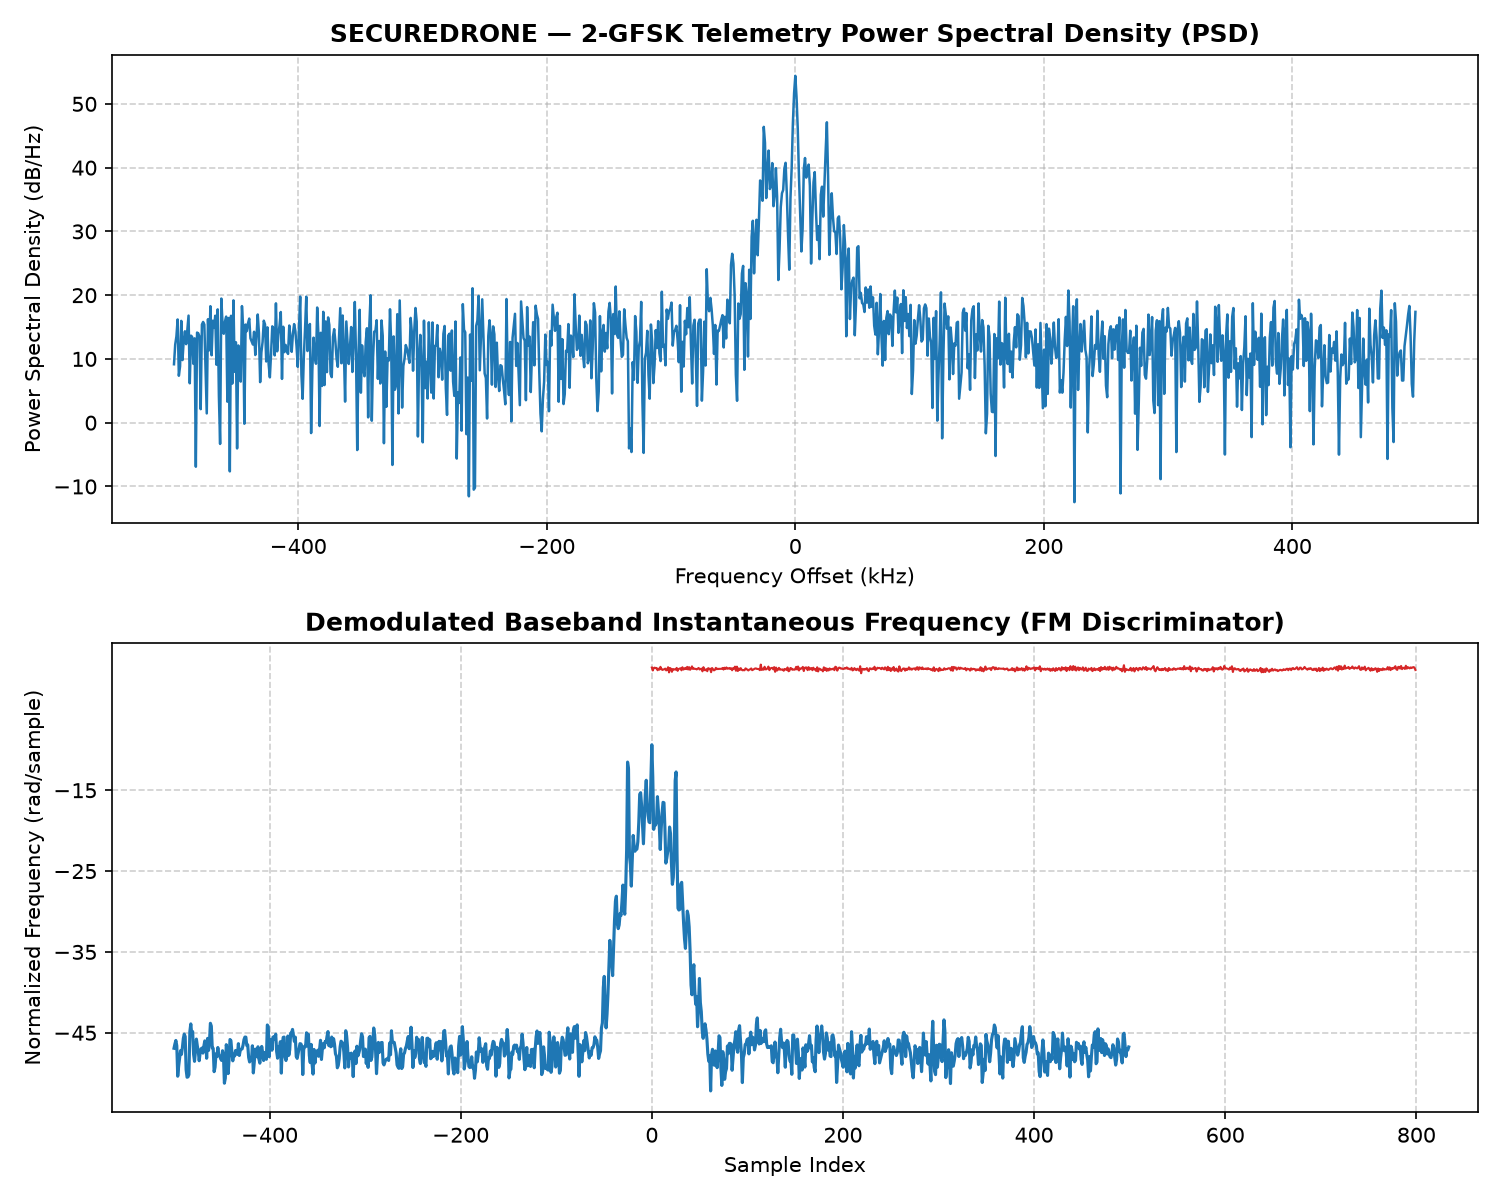
\includegraphics[width=0.85\textwidth]{evidence/rf_demodulation_plot.png}
    \caption{Power Spectral Density (PSD) and Baseband FM Discriminator Output}
    \label{fig:rf_demod}
\end{figure}

\subsection{GNSS Cyber-Physical Spoofing Anomaly Detection}
In \texttt{navigation-security/anomaly-detection/detector.py}, I investigated UAV state estimation resilience against two realistic GNSS spoofing profiles across a 1,000-epoch flight trajectory:
\begin{enumerate}
    \item \textbf{Attack 1 (Sudden Step Spoofing)}: Abrupt $+65\text{ m}$ position offset ($t = 30\dots 45\text{ s}$).
    \item \textbf{Attack 2 (Coordinated Drift Spoofing)}: Quadratic position drift accelerating at $0.35\text{ m/s}^2$ ($t = 60\dots 85\text{ s}$).
\end{enumerate}

To protect the vehicle, I implemented a two-tier kinematic integrity detector:
\begin{itemize}
    \item \textbf{Tier 1: EKF Chi-Square Innovation Filter ($\chi^2$)}: Measures second-order extrapolation residuals normalized by innovation variance $\sigma_{\text{innov}}^2 = 6\sigma^2$:
    \begin{equation}
        \chi^2[k] = \frac{(x[k] - 2x[k-1] + x[k-2])^2 + (y[k] - 2y[k-1] + y[k-2])^2}{6\sigma^2}
    \end{equation}
    When $\chi^2[k] > 9.21$ (99\% confidence threshold), the filter rejects the measurement and transitions to \texttt{ALT\_HOLD} (Inertial Dead-Reckoning).
    \item \textbf{Tier 2: CUSUM Statistical Drift Filter}: Accumulates small, persistent bias deviations that evade instantaneous thresholds:
    \begin{equation}
        S[k] = \max\Big(0, \lambda S[k-1] + \Delta_{\text{dist}}[k] - v_{\text{nom}}\Delta t - \text{slack}\Big)
    \end{equation}
    When $S[k] > 10.0$, the vehicle identifies coordinated drift and triggers \texttt{AUTO\_LAND}.
\end{itemize}

\begin{figure}[htbp]
    \centering
    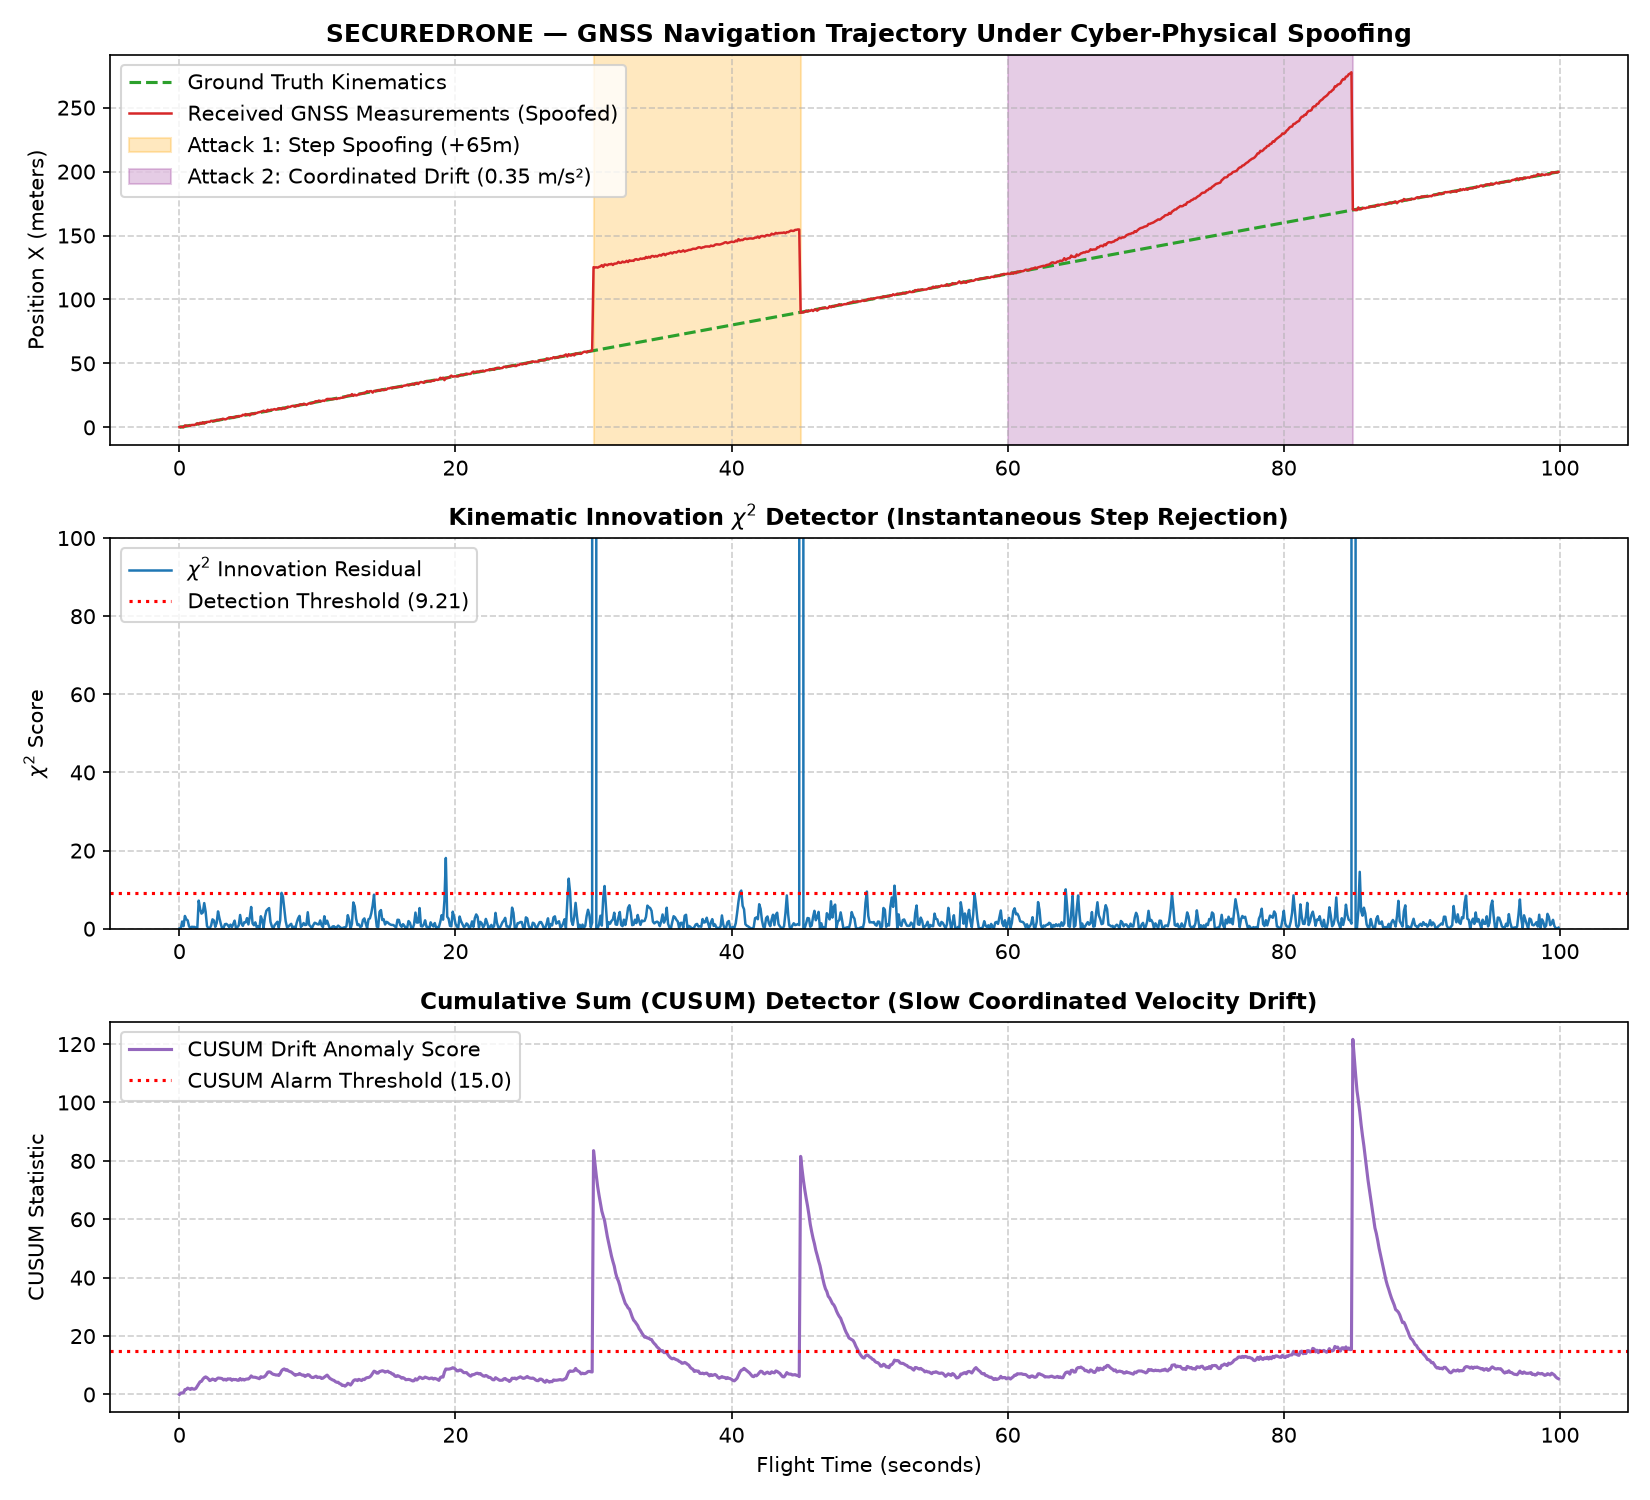
\includegraphics[width=0.85\textwidth]{evidence/gnss_anomaly_detection_plot.png}
    \caption{GNSS Spoofing Trajectory, Innovation Residuals, and CUSUM Drift Response}
    \label{fig:gnss_plot}
\end{figure}

\begin{table}[htbp]
    \centering
    \small
    \begin{tabular}{lll}
        \toprule
        \textbf{Metric} & \textbf{Observed Benchmark} & \textbf{Defensive Outcome} \\
        \midrule
        Step Attack Time-to-Detect (TTD) & \textbf{0 ms} (Immediate) & Triggered Altitude Hold (\texttt{ALT\_HOLD}) \\
        Drift Attack Time-to-Detect (TTD) & \textbf{21.7 seconds} & Triggered Controlled Landing (\texttt{AUTO\_LAND}) \\
        Baseline False Alarm Rate & \textbf{1.03\%} & Safe operational tolerance ($< 2\%$) \\
        \bottomrule
    \end{tabular}
    \caption{GNSS Integrity Detection Performance Benchmark}
    \label{tab:gnss_metrics}
\end{table}

% -----------------------------------------------------------------------------
\section{Stage 06: Formal Findings Register \& Verification Matrix}
% -----------------------------------------------------------------------------

\subsection{Vulnerability Findings Register}
\begin{enumerate}
    \item \textbf{SEC-MAV-001 (CVSS 8.8 --- High)}: Cleartext, unauthenticated telemetry and command execution on UDP port 14550.
    \item \textbf{SEC-MAV-002 (CVSS 8.1 --- High)}: Bit-for-bit command replay susceptibility due to lack of monotonic timestamp validation.
    \item \textbf{ARCH-MAV-001 (CVSS 6.8 --- Medium)}: Absence of non-repudiation in MAVLink 2 symmetric signing; peripheral compromise yields GCS command forgery.
    \item \textbf{SEC-CMP-001 (CVSS 9.8 --- Critical)}: Remote command injection and unauthenticated MAVLink command dispatch on companion API.
    \item \textbf{SEC-NAV-001 (CVSS 7.5 --- High)}: Susceptibility to unauthenticated GNSS signal manipulation resulting in flight path deviation.
\end{enumerate}

\subsection{Automated Regression Verification}
To guarantee reproducible defense, all modules are covered by automated \texttt{pytest} regression test suites:
\begin{lstlisting}[language=bash]
PYTHONPATH=. pytest mavlink-security/tests/ companion-security/tests/ \
    firmware-analysis/unpackers/test_unpacker.py \
    rf-analysis/signal-processing/test_rf_demod.py -v
\end{lstlisting}
\begin{table}[htbp]
    \centering
    \small
    \begin{tabular}{lll}
        \toprule
        \textbf{Test Module} & \textbf{Property Verified} & \textbf{Result} \\
        \midrule
        \texttt{test\_parse\_mavlink\_v1\_synthetic} & MAVLink v1 framing \& CRC parsing & \textbf{PASS} \\
        \texttt{test\_parse\_mavlink\_v2\_synthetic} & MAVLink v2 24-bit message IDs & \textbf{PASS} \\
        \texttt{test\_parse\_mavlink\_v2\_signed} & 13-byte signature trailer extraction & \textbf{PASS} \\
        \texttt{test\_parse\_baseline\_pcap} & 3,748-frame live PCAP dissection & \textbf{PASS} \\
        \texttt{test\_firewall\_blocks\_critical} & MAVLink Firewall drops command ID 185/400 & \textbf{PASS} \\
        \texttt{test\_firewall\_permits\_safe} & MAVLink Firewall permits velocity setpoints & \textbf{PASS} \\
        \texttt{test\_hardened\_api\_auth} & Rejection of unauthenticated HTTP requests & \textbf{PASS} \\
        \texttt{test\_firmware\_vector\_table} & Cortex-M7 SP in SRAM, Reset in Flash & \textbf{PASS} \\
        \texttt{test\_gfsk\_demod\_and\_crc} & Quadrature demodulation \& CRC-16-CCITT & \textbf{PASS} \\
        \texttt{test\_gnss\_anomaly\_detection} & Multi-layer step \& drift spoofing rejection & \textbf{PASS} \\
        \midrule
        \textbf{Total Regression Suite} & \textbf{13 Test Cases Evaluated} & \textbf{13 / 13 PASS (100\%)} \\
        \bottomrule
    \end{tabular}
    \caption{Defensive Engineering Automated Verification Summary}
    \label{tab:tests}
\end{table}

% -----------------------------------------------------------------------------
\section{Conclusion}
% -----------------------------------------------------------------------------
The \textbf{SECUREDRONE} platform demonstrates that empirical, end-to-end cybersecurity assessments of unmanned systems provide insights that cannot be captured by isolated software auditing alone. By evaluating the system across network protocols, companion software, embedded firmware, RF modulation, and cyber-physical navigation loops, I uncovered critical architectural trust-boundary weaknesses and implemented working, verified mitigations. 

All code, PCAP captures, firmware manifests, signal processing pipelines, and formal reports are preserved in the repository for peer reproduction, open-source publication, and technical portfolio demonstration.

\end{document}
